\documentclass[oneside,10pt]{book}
%\reversemarginpar
%\usepackage{geometry}
%\newgeometry{a4paper,top=2.5cm,left=1.2in,right=1.2in,headheight=1cm,headsep=0.5cm,marginpar=2.6cm,
%marginparsep=10pt,textheight=49\baselineskip}

\usepackage{lipsum,pgf,caption}
\usepackage{tikz}
\usetikzlibrary{decorations,decorations.shapes,shapes,fadings,patterns}
     % We need lots of libraries...
        \usetikzlibrary{
          arrows,
          calc,
          fit,
          patterns,
          plotmarks,
          shapes.geometric,
          shapes.misc,
          shapes.symbols,
          shapes.arrows,
          shapes.callouts,
          shapes.multipart,
%          shapes.gates.logic.US,
%          shapes.gates.logic.IEC,
%          circuits.logic.US,
%          circuits.logic.IEC,
%          circuits.logic.CDH,
%          circuits.ee.IEC,
%          datavisualization,
          datavisualization.formats.functions,
          er,
          automata,
          backgrounds,
          chains,
          topaths,
          trees,
          petri,
          mindmap,
          matrix,
          calendar,
          folding,
          fadings,
          shadings,
          spy,
          through,
          turtle,
          positioning,
          scopes,
          decorations.fractals,
          decorations.shapes,
          decorations.text,
          decorations.pathmorphing,
          decorations.pathreplacing,
          decorations.footprints,
          decorations.markings,
          shadows,
%          lindenmayersystems,
          intersections,
          fixedpointarithmetic,
          fpu,
          svg.path,
%          external,
        }


\IfFileExists{changepage.sty}{%
  \PassOptionsToPackage{strict}{changepage}
  \RequirePackage{changepage}
  }{}
%\usepackage[strict]{changepage}
\def\aspectratio{\pgfmathparse{\paperheight/\paperwidth} \pgfmathresult}
\newpage
\newlength\innermargin

\def\printgeometryvalues{\leavevmode
paperwidth \the\paperwidth\\
paperheight \the\paperheight\\
theheadheight \the\headheight\\
theheadsep \the\headsep\\
thetopmargin \the\topmargin\\
theoddsidemargin \the\oddsidemargin\\
theevensidemargin\the\evensidemargin\\
thetextheight\the\textheight\\
thetextwidth \the\textwidth\\
themarginparsep \the\marginparsep\\
themarginparwidth \the\marginparwidth\\
themarginpush \the\marginparpush\\
thevoffset \the\voffset
thefootskip \the\footskip\\
aspect ratio \aspectratio\\
topskip \the\topskip\par}

\def\alignedge{%
  \checkoddpage%
  \parindent0pt%
   \ifoddpage \global\setlength\innermargin{\oddsidemargin}
          \else \global\setlength\innermargin{\evensidemargin}
      \fi%
   \if@twoside\setlength\innermargin{\dimexpr(\evensidemargin-\marginparsep)}%
             \else\let\innermargin\oddsidemargin\fi
 }

\parindent0pt

%\pagecolor{brown}
%\color{white}
\begin{document}
\mainmatter
\fboxsep0pt\fboxrule0pt
%\checkoddpage

\def\topofpageimage#1{%
\clearpage
\alignedge
\vspace*{\dimexpr(1in+\headheight+\headsep+\topmargin+\topskip)*(-1)}
\hspace*{\dimexpr(-1in-\innermargin)}%
\fbox{\includegraphics[width=\paperwidth]{./chapters/#1}}\par
\medskip}

\topofpageimage{hine01}
\printgeometryvalues


% First example
\topofpageimage{hine02}
\printgeometryvalues
\lipsum


% Second example
\topofpageimage{hine03}
\printgeometryvalues\marginpar{testing}
\lipsum\marginpar{testing}
\lipsum[1-20]


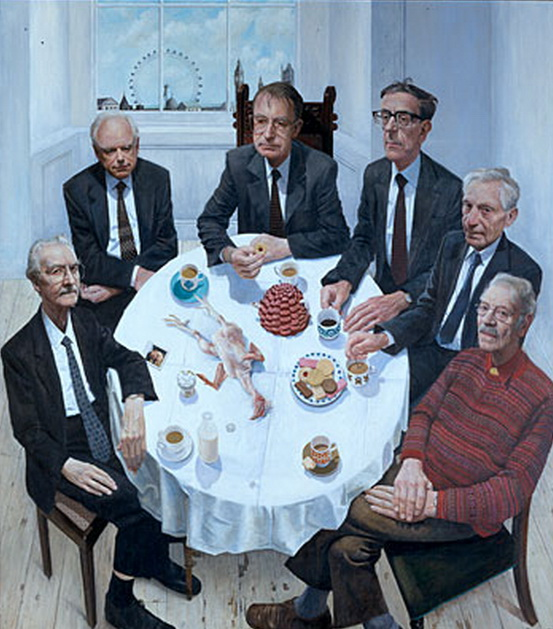
\includegraphics[height=\textheight]{stuartpearson}
\clearpage

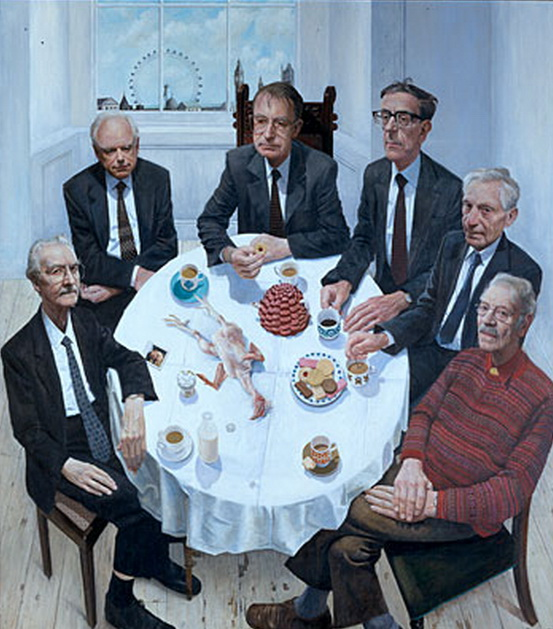
\includegraphics[height=\textheight]{stuartpearson}


\restoregeometry

\newpage \newpage

\def\tol{3mm}
\def\printlayout{
\begin{tikzpicture}[scale=0.5,font={\footnotesize\sffamily}]
\coordinate (pageX1) at (0,\paperheight);
\coordinate (text1) at (1in+\innermargin,\paperheight-1in-\headsep-\headheight);
% origin
\draw [fill=black] (0,0) circle (3.5pt); 
% draw paper
\draw [color=red] (pageX1) rectangle ++(\paperwidth, -\paperheight);
% draw one inch around
\draw [color=gray] (1in, 0) -- ++(0, \paperheight);
\draw [color=gray] (0, \paperheight-1in) -- ++ (\paperwidth,0);
% draw textarea
\draw [color=green] (text1) rectangle ++ (\textwidth ,-\textheight);
% oddside margin
\draw [color=blue] (1in+\innermargin, \paperheight-1in-\headsep-\headheight) -- ++ (0,-\textheight);
% marginpar
\draw [color=blue] (1in+\innermargin+\textwidth+\marginparsep,\paperheight-1in-\headsep-\headheight ) rectangle ++(\marginparwidth,-\textheight);
% header
\draw [color=black, line width=1.5pt] (1in + \innermargin, \paperheight-1in-\headheight) -- ++ (\textwidth,0) rectangle ++ (0, \headheight);
% footer
\draw (1in+\innermargin,\paperheight-1in-\headheight-\headsep-\textheight-\footskip)
         -- ++ (\textwidth,0);
% legends and dimensions
\draw (0,\paperheight+\tol) -- ++(0,.8) ++ (1in, -0.8) -- ++(0,.8) ++ (\paperwidth-\textwidth,-.8) -- ++ (0,.8) ++ (\marginparsep, -0.8) -- ++(0, 0.8) ++ (\marginparwidth, -0.8) -- ++ (0, 0.8) (\paperwidth,\paperheight+\tol)--++(0,0.8);
\draw (-0.4,\paperheight+3mm+4mm) -- ++ (\paperwidth+8mm,0);
% on y-axis right
\draw (\paperwidth+\tol,\paperheight)
        -- ++ (0.8,0)
        ++ (-0.8,-1in)--++(0.8,0)
        ++ (-0.8,-\headheight)-- ++(0.8,0)
        ++ (-0.8,-\headsep) -- ++ (0.8,0)
        ++ (-0.8,-\textheight) -- ++ (0.8,0)
        ++ (-0.8, -\footskip) -- ++ (0.8,0)
        (\paperwidth+7mm,\footskip-3mm)-- ++ (0,\paperheight+0.4);  
% bottom dimensions
\draw (-3mm,- 10mm) -- ++(1in+1cm,0) node[above] at ++(-0.5in-0.5cm,0){1 inch}(1in,-8.3mm)--++(0,-0.8cm);  
\draw (0,-8mm)-- 
       ++(0, -2.5cm)++(\paperwidth,2.5cm)--++(0,-2.5cm); 
\draw (-3mm,-2.5cm)--++(\paperwidth+6mm,0);
\node[above] at (-3mm+0.5\paperwidth, -2.5cm) {paper width = \the\paperwidth};  
%% left tick marks
\draw (-3mm,0)-- (-1.3cm,0)++(-3mm,\paperheight)--++(1cm,0);
\draw (-7.5mm, -0.4) -- ++ (0,\paperheight+ 1.2);
\end{tikzpicture}

\clearpage
\printgeometryvalues}

\printlayout

\printlayout

\end{document} 